\section{Ekran dodawania danych}
\sectionauthor{R. Wolniak}

Głównym wyzwaniem okazał się brak systematycznej organizacji danych w arkuszach programu
Excel, co skutkowało niekompatybilnością z zaprojektowaną bazą danych. W celu rozwiązania tego
problemu opracowano dedykowany interfejs w aplikacji, który wspomaga użytkownika w procesie
przetwarzania danych, minimalizując ryzyko wystąpienia błędów. Składa się on z:
\begin{itemize}
    \item sekcji pozwalającej użytkownikowi na zapisanie pliku w chmurze,
    \item formularza walidacji nazw kolumn,
    \item kontrolek umożliwiających wybór roku i numeru indykacji oraz przycisku do przesłania danych do bazy,
    \item formularza do uzupełniania lub edycji numerów MPK.
\end{itemize}

% \noindent Rysunek \ref{fig:managedatascreen} przedstawia finalny wygląd ekranu dodawania danych do systemu. Komponenty znajdujące się na ekranie zostały opisane poniżej.
% \begin{figure}[H]
%     \centering
%     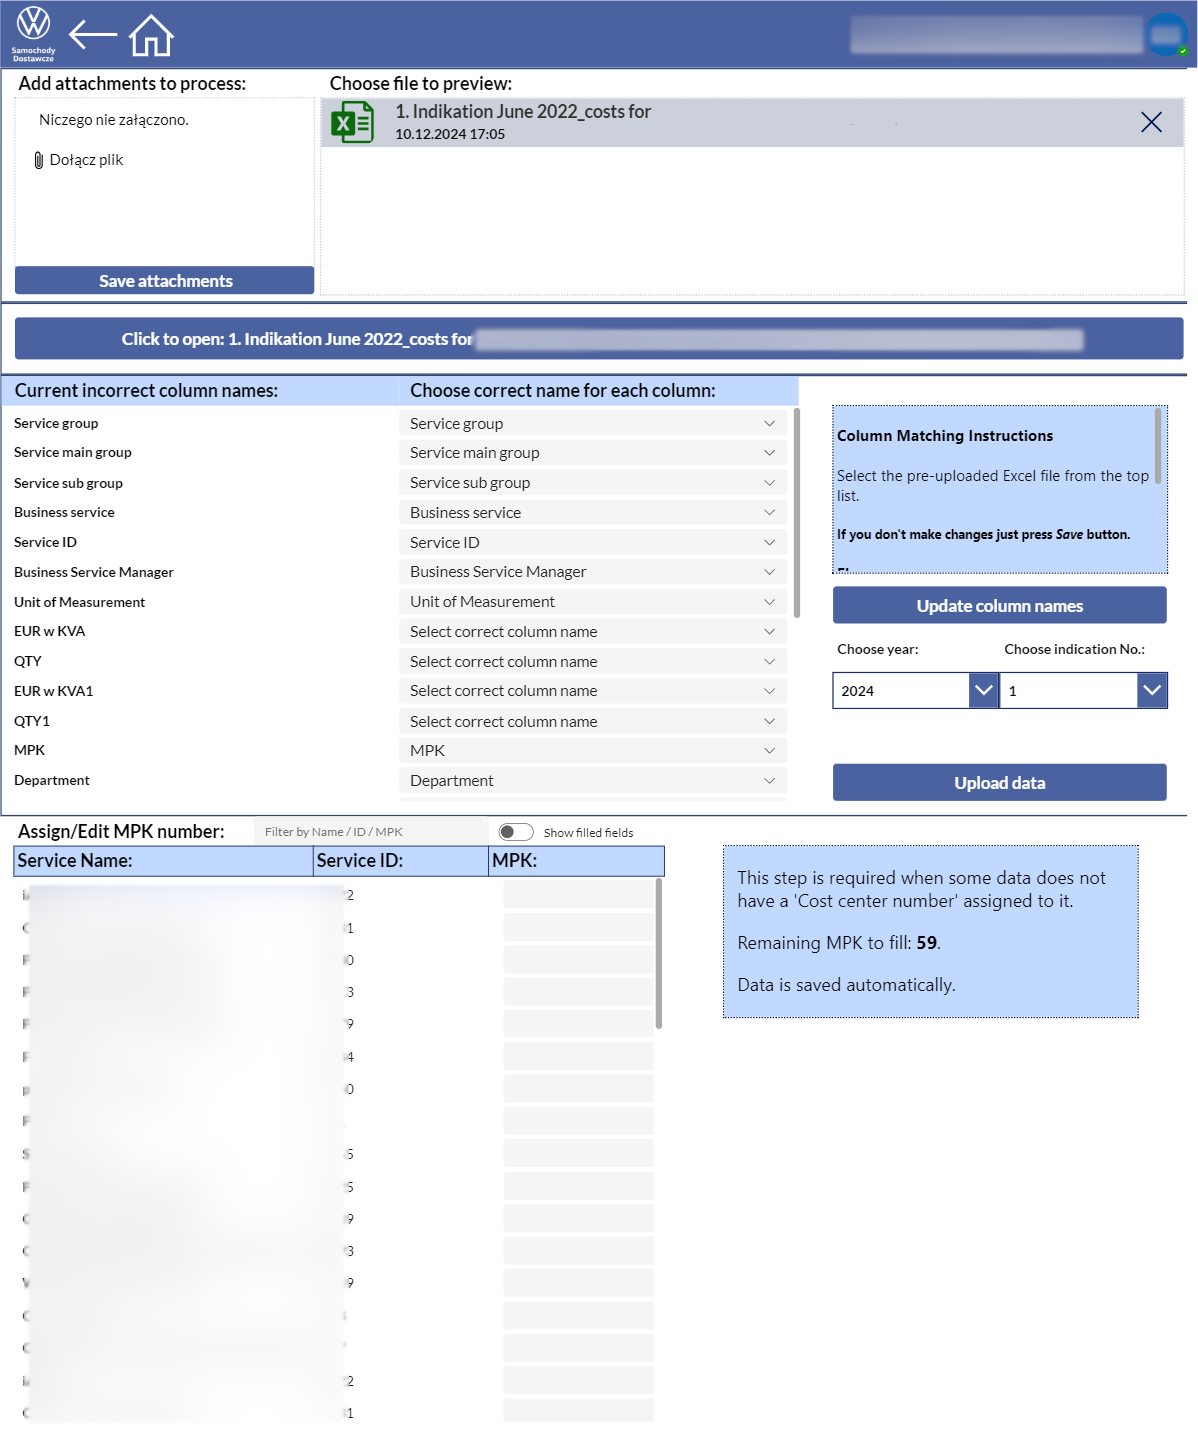
\includegraphics[width=0.9\textwidth]{figures/ManageDataScreen.png}
%     \caption{Ekran dodawania danych do systemu} 
%     \label{fig:managedatascreen}
% \end{figure}

\subsection{Zapis pliku w chmurze}
Pierwszym etapem procesu jest tymczasowy zapis pliku Excel w chmurze, co umożliwia jego udostępnienie innym systemom. Do realizacji tego zadania wykorzystano kontrolkę\footnote{Kontrolka -- element służący do nawigacji, wyświetlania danych i obsługi aplikacji.} \emph{Attachment Control}. Pozwala ona na zapisanie pliku w pamięci aplikacji. Odbywa się to przez naciśnięcie przycisku \emph{"Attach file"} lub przy użyciu mechaniki \emph{przeciągnij i upuść} (\english{Drag And Drop}).

Pod kontrolką \emph{Attachment Control} dodano przycisk \emph{Save attachment}. Jego naciśnięcie skutkuje wywołaniem szeregu funkcji opisanych we właściwości \emph{OnSelect}:
\begin{itemize}
    \item spawdzenie czy plik został poprawnie załadowany,
    \item wywołanie przepływu \emph{SaveFileAndRunScript},
    \item zapisanie wyniku przepływu w zmiennej tablicowej \emph{FlowOutput} (w Power Apps określanej jako \emph{kolekcja}),
    \item po poprawnym zapisaniu pliku w folderze SharePoint, usunięcie go z pamięci aplikacji.
\end{itemize}

% Aby dalej przekazać plik oraz jego zawartość należy nacisnąć przycisk opisany jako \emph{Save attachments} znajdujący się pod wcześniej omawianym elementem. Naciśnięcie go skutkuje wywołaniem szeregu funkcji opisanych we właściwości \emph{OnSelect}. W pierwszej kolejności sprawdzane jest, czy plik został załadowany. Jeśli tak, to wywoływany jest przepływ \emph{SaveFileAndRunScript}. Wynik przepływu jest zapisywany w zmiennej tablicowej, która w Power Apps określana jest jako \definicja{kolekcja}, o nazwie \emph{FlowOutput}. Po wykonaniu się przepływu, pliki zapisane w folderze SharePoint, zostają usunięte z pamięci aplikacji.



\subsubsection*{Przepływ SaveFileAndRunScript}
\label{childflow}
Rysunek \ref{fig:savefileandrunscript} przedstawia edytor programu Power Automate. Widoczny w nim przepływ nazwany \emph{SaveFileAndRunScript} jest odpowiedzialny za zapisanie pliku w chmurze oraz wstępne przetworzenie. W momencie wywołania przepływu plik zostaje przekazany jako parametr wejściowy. Przepływ ten składa się z kilku kroków, które zostaną omówione w kolejności ich wykonywania.

\begin{figure}[t]
    \centering
    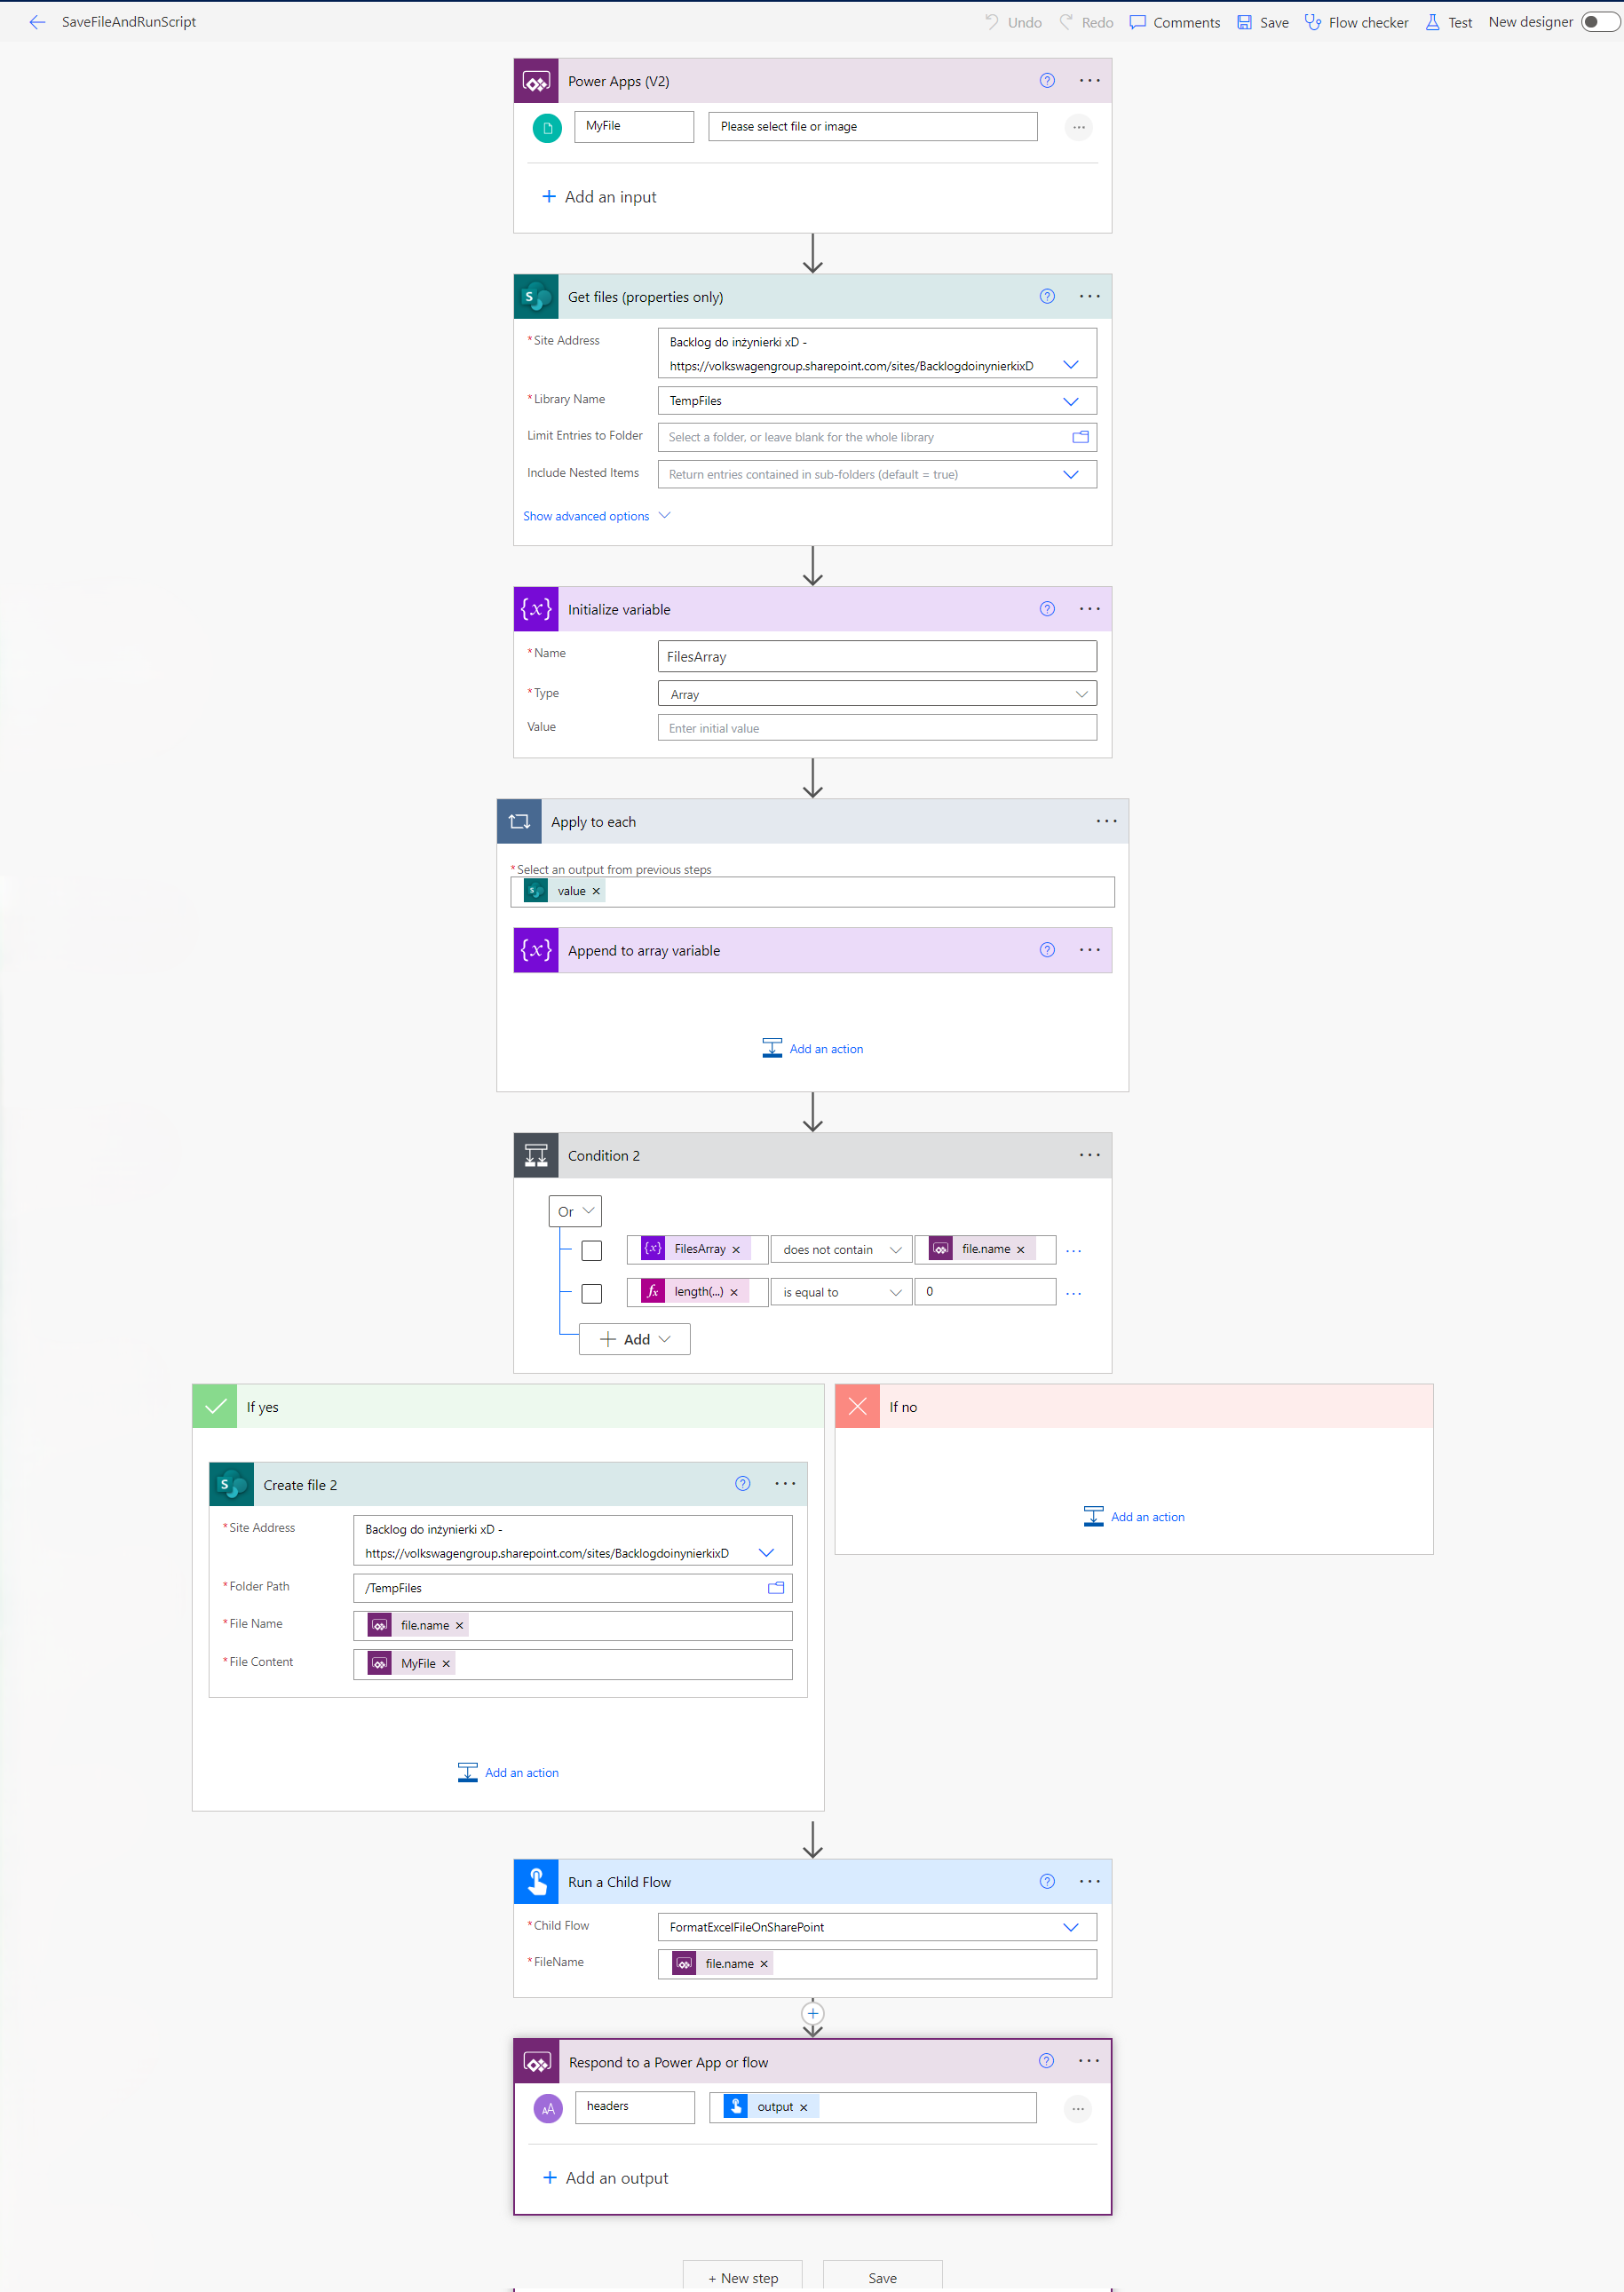
\includegraphics[width=0.9\textwidth]{figures/SaveFileAndRunScript.png}
    \caption{Widok przepływu SaveFileAndRunScript}
    \label{fig:savefileandrunscript}
\end{figure}


\begin{enumerate}
    \item \textbf{Funkcja: Power Apps (V2)} \\
          Przepływ rozpoczyna się od funkcji oczekującej na wywołanie przepływu bezpośrednio z aplikacji Power Apps. Jako parametry wejściowe przyjmuje:
          \begin{itemize}
              \item nazwę pliku (\textit{File Name}),
              \item zawartość pliku (\textit{File Content}) w formacie binarnym.
          \end{itemize}

    \item \textbf{Zainicjowanie zmiennej} \\
          Element \textit{Initialize variable} tworzy zmienną o nazwie \textit{FileExists}, która przechowuje informację o tym, czy plik o podanej nazwie znajduje się już na SharePoint.

    \item \textbf{Sprawdzenie istniejących plików} \\
          Blok \textit{Get files} pobiera listę wszystkich plików z wybranego folderu SharePoint wraz z ich metadanymi, takimi jak nazwa, ścieżka czy data modyfikacji. Wynik zostaje zapisany w zmiennej \textit{FileExists}, która przyjmuje wartość \textit{true}, jeśli plik został znaleziony, lub \textit{false}, jeśli plik nie istnieje.

    \item \textbf{Instrukcja warunkowa \emph{If}} \\
          Element \textit{Condition} sprawdza wartość zmiennej \textit{FileExists}. W zależności od wyniku:
          \begin{itemize}
              \item jeśli zmienna ma wartość \textit{true} -- przepływ kończy działanie,
              \item jeśli zmienna ma wartość \textit{false} -- przepływ kontynuuje proces zapisu.
          \end{itemize}

    \item \textbf{Utworzenie pliku} \\
          Blok \textit{Create file} tworzy nowy plik w SharePoint, wykorzystując parametry:
          \begin{itemize}
              \item adres witryny SharePoint,
              \item ścieżkę do folderu docelowego,
              \item nazwę pliku,
              \item zawartość pliku.
          \end{itemize}

    \item \textbf{Uruchomienie przepływu podrzędnego} \\
          Po pomyślnym zapisaniu pliku przepływ wywołuje tzw. \textit{child flow}, które inicjuje działanie skryptu Office. Skrypt ten odpowiada za przetworzenie pliku w sposób zgodny z założeniami aplikacji. Jego wynik w formacie JSON jest zwracany do strumienia nadrzędnego.

    \item \textbf{Odpowiedź do aplikacji} \\
          Blok \textit{Respond to Power Apps} kończy przepływ, zwracając do aplikacji dane w formacie JSON, przetworzone przez wspomniany skrypt.
\end{enumerate}

\subsection{Skrypt pakietu Office}
Po utworzeniu pliku w SharePoint, w ramach przepływu następuje jego przetworzenie przez skrypt. Jest to niezbędne, jeśli chodzi o działanie procesu. Domyślnie otrzymane dane w pliku Excel są niewidoczne dla większości systemów, mogą one odczytać jedynie informacje zorganizowane w \emph{tabele programu Excel}\footnote{Tabela w programie Excel wymaga osobnej deklaracji poprzez zaznaczenie zakresu komórek i wybór opcji \emph{Narzędzia główne}$\to$\emph{Formatuj jako tabelę}}, w związku z tym powstał skrypt, który działa bezpośrednio w arkuszu. Jego zadaniem jest automatyczne utworzenie tabeli oraz dostosowanie jej do wymagań systemu. Poniżej przedstawiono kroki działania skryptu:

\begin{enumerate}
    \item \textbf{Wybór arkusza roboczego} \\
          Skrypt identyfikuje arkusz zawierający dane, analizuje zakres używanych komórek i usuwa zabezpieczenie pliku przed edycją, jeśli jest aktywne -- krok ten jest wymagany, aby wprowadzanie zmian w arkuszu było możliwe.

    \item \textbf{Analiza danych} \\
          Skrypt rozpoczyna analizę od wyszukiwania początku tabeli w arkuszu. Następnie:
          \begin{itemize}
              \item usuwa puste kolumny, które nie zawierają żadnych danych,
              \item tworzy tabelę o dynamicznym rozmiarze, uwzględniając zakres danych znajdujących się w arkuszu,
              \item uzupełnia brakujące komórki w przypadku kolumn /emph{Service group}, /emph{Service main group}, /emph{Service sub group}, korzystając z danych z poprzednich wierszy.
          \end{itemize}
          Takie podejście pozwala na uporządkowanie danych i przygotowanie ich do dalszego przetwarzania.

    \item \textbf{Dopasowanie nazw kolumn} \\
          Skrypt porównuje istniejące nazwy kolumn z listą standardowych nagłówków, korzystając z algorytmu \textit{Jaro-Winkler}. Algorytm ten:
          \begin{itemize}
              \item analizuje podobieństwo tekstów, porównując wspólne znaki oraz ich kolejność,
              \item przyznaje dodatkowe punkty za zgodność początkowych znaków (prefiksu),
              \item zwraca wynik jako wartość z przedziału od 0 do 1, gdzie wartości bliższe 1 oznaczają większe podobieństwo.
          \end{itemize}
          Wynik tego procesu jest wykorzystywany w dalszych etapach aplikacji, m.in. do walidacji struktury danych. Jeśli podobieństwo jest mniejsze niż 90\%, skrypt sugeruje ręczne dopasowanie nazwy kolumny.

    \item \textbf{Zwrócenie wyników} \\
          Skrypt generuje JSON zawierający mapowanie oryginalnych nazw kolumn z najlepszymi dopasowaniami z listy standardowych nagłówków.
\end{enumerate}


Kolejnym elementem tej sekcji ekranu jest lista zapisanych plików znajdująca się obok kontrolki \emph{Attach Control}. Umożliwia ona wybór pliku do dalszego przetwarzania. Poniżej umieszczono przycisk \emph{"Click to open:..."}, który pozwala na otwarcie wybranego pliku w nowym oknie przeglądarki przy użyciu funkcji \emph{Launch}. Możliwość podglądu ma na celu ułatwienie weryfikacji jego poprawności.

\subsubsection*{Algorytm Jaro-Winkler}
Podstawą algorytmu jest algorytm \emph{Jaro}. Polega on na porównaniu dwóch ciągów znaków w celu określenia ich podobieństwa. Wynik obliczany jest na podstawie równania \ref{eq:Jaro}:
\begin{equation}
    \label{eq:Jaro}
    J = \frac{1}{3} \left( \frac{m}{|s_1|} + \frac{m}{|s_2|} + \frac{m - t}{m} \right) \mbox{dla } m>0
\end{equation}
\noindent gdzie:\\
$m$ – liczba dopasowanych znaków,\\    $t$ – liczba transpozycji,\\    $|s_1|$, $|s_2|$ – długości ciągów.\\

\noindent Wynikiem równania, jest wartość z przedziału od 0 do 1, gdzie 1 oznacza pełne dopasowanie.

Algorytm \emph{Jaro-Winkler} jest rozszerzeniem algorytmu \emph{Jaro}, które dodaje premię za zgodność początkowych znaków. Wynik obliczany jest na podstawie równania \ref{eq:JaroWinkler}:
\begin{equation}
    \label{eq:JaroWinkler}
    JW = J + l \cdot p \cdot (1 - J),
\end{equation}
gdzie:\\
$l$ – długość wspólnego prefiksu (maksymalnie 4 znaki),\\ $p$ – współczynnik skalowania.\\

\noindent Rozszerzona wersja algorytmu pozwala na bardziej precyzyjne porównanie ciągów znaków, które mają wspólny prefiks, co jest szczególnie ważne w przypadku nagłówków kolumn rozpoczynających się od frazy \emph{Service}.


\vspace{1cm}

% \textcolor{red}{LINK DO TEGO JARO\_WINKLERA: https://crucialbits.com/blog/a-comprehensive-list-of-similarity-search-algorithms/
% https://en.wikipedia.org/wiki/Jaro\%E2\%80\%93Winkler\_distance
% }


\subsection{Walidacja nazw kolumn} Kolejnym etapem, przed zapisaniem danych do bazy, jest walidacja nazw kolumn. W tym celu zaimplementowano formularz zawierający \emph{galerię} -- element umożliwiający wyświetlanie wielu rekordów danych o różnych typach. Pola wyświetlające dane w galerii mogą być dostosowywane w dowolny sposób, w zależności od potrzeb użytkownika.

\noindent Galeria składa się z dwóch kolumn:
\begin{itemize}
    \item Lewej, prezentującej obecne nazwy kolumn, które są wyświetlane za pomocą kontrolki \emph{Label}\footnote{\emph{Label} -- kontrolka tekstowa, umożliwiająca wyświetlanie statycznych wartości.}.
    \item Prawej, zawierającej kontrolkę \emph{ComboBox}\footnote{\emph{ComboBox} -- rozwijana lista z możliwością wprowadzania tekstu}, która umożliwia wybór nazwy ze standardowej listy nagłówków. Wartości domyślne, widoczne w kontrolkach \emph{ComboBox}, są generowane przez wcześniej opisany skrypt w taki sposób, aby do oryginalnej nazwy kolumny dopasowana została najbardziej podobna nazwa z predefiniowanej listy nagłówków. Ma to na celu minimalizację danych wprowadzonych przez użytkownika.
\end{itemize}

Po prawej stronie formularza umieszczono instrukcję użytkownika, zawierającą wskazówki dotyczące prawidłowego uzupełniania nazw kolumn. Poniżej instrukcji dodano przycisk \emph{Update column names}, który umożliwia zapisanie zmian w strukturze danych.

\noindent Działanie tego mechanizmu opiera się na zastosowaniu skryptu pakietu Office, wywoływanego przy użyciu kolejnego przepływu. Skrypt, jako parametr wejściowy, przyjmuje zmienną tablicową w formacie JSON, zawierającą mapowanie oryginalnych nazw kolumn z poprawionymi wartościami wybranymi przez użytkownika. Następnie skrypt iteruje po wierszu zawierającym nagłówki kolumn i dokonuje ich zamiany zgodnie z otrzymaną mapą. Po zakończeniu działania skrypt zwraca nową strukturę nazw kolumn.

Pod przyciskiem \emph{Update column names} umieszczone zostały kontrolki \emph{Dropdown}\footnote{\emph{Dropdown} -- kontrolka umożliwiająca wybór jednej z dostępnych wartości z rozwijanej listy, bez możliwości edycji.} oraz przycisk \emph{Upload data}, które są kluczowe dla kolejnego etapu przetwarzania danych, obejmującego ich integrację z listami SharePoint.


% \begin{figure}[t]
%     \centering
%     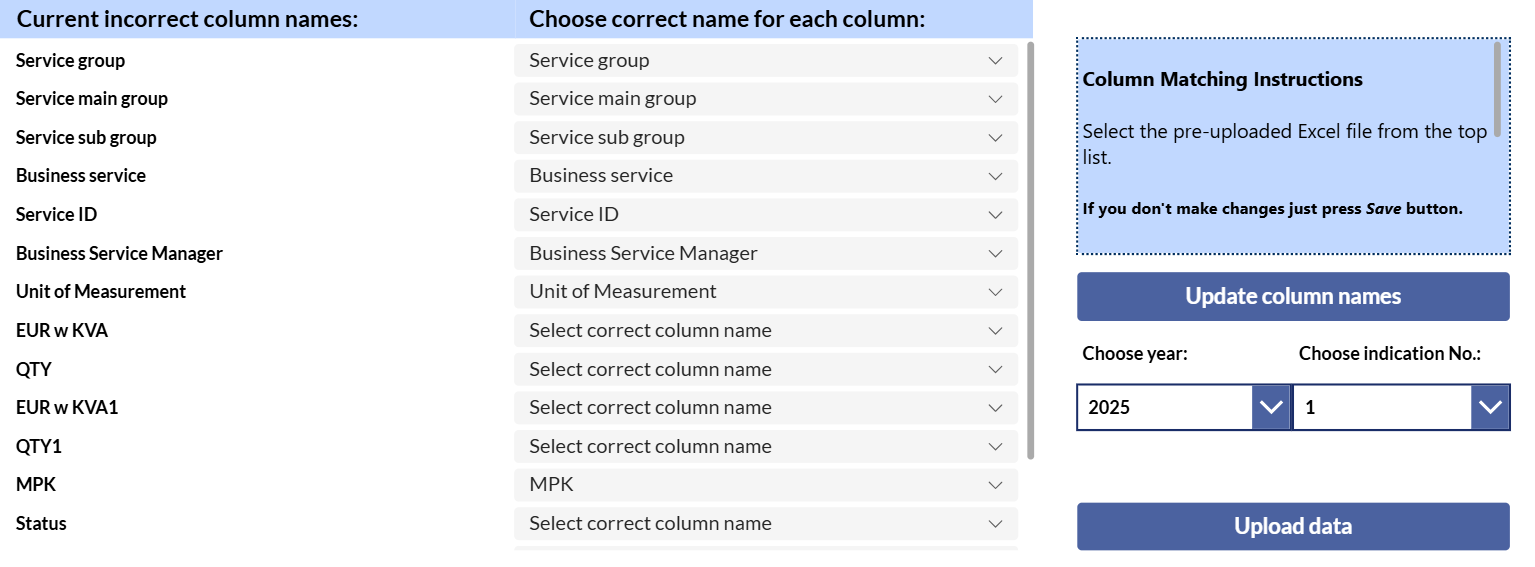
\includegraphics[width=\textwidth]{figures/ColumnMappingForm.png}
%     \caption{Formularz walidacji nazw kolumn}
%     \label{fig:columnmappingform}
% \end{figure}

\subsection{Integracja z listami SharePoint} Po zakończeniu walidacji nazw kolumn, kolejnym etapem jest zapisanie przetworzonych danych w utworzonej strukturze SharePoint. Proces ten rozpoczyna się od wyboru roku i numeru indykacji przy użyciu dedykowanych kontrolek \emph{Dropdown}. Wybrane wartości są następnie wykorzystywane podczas importu danych do odpowiednich list, co odbywa się za pomocą przycisku \emph{Upload data}.

Skutki kliknięcia przycisku mogą różnić się w zależności od wybranych wartości i tego czy nazwy kolumny zostały zmienione. Jeśli przed próbą wgrania danych nie został wciśnięty przycisk \emph{Update column names}, system wyświetla okno z zapytaniem o poprawność nazw kolumn w celu upewnienia się, że użytkownik nie wgra przypadkowo danych z niepoprawnymi nagłówkami.
Jeśli jednak nazwy kolumn zostały zmienione, a użytkownik wybierze rok oraz numer indykacji istniejące w bazie danych, system wyświetli zapytanie, czy użytkownik chce nadpisać istniejące dane, czy anulować operację. W momencie gdy nazwy kolumn nie zostaną zmienione, a dane z wybranym rokiem i numerem indykacji istnieją w bazie danych, wyświetlą się oba okna z informacjami.


% Rysunki \ref{fig:CorrectHeadersPopup} oraz \ref{fig:DoYouWantToOverwrite} przedstawiają dwa możliwe scenariusze, które mogą wystąpić po naciśnięciu przycisku.
% \begin{figure}[htbp]
%     \centering
%     % Pierwszy obrazek
%     \begin{minipage}{0.48\textwidth}
%         \centering
%         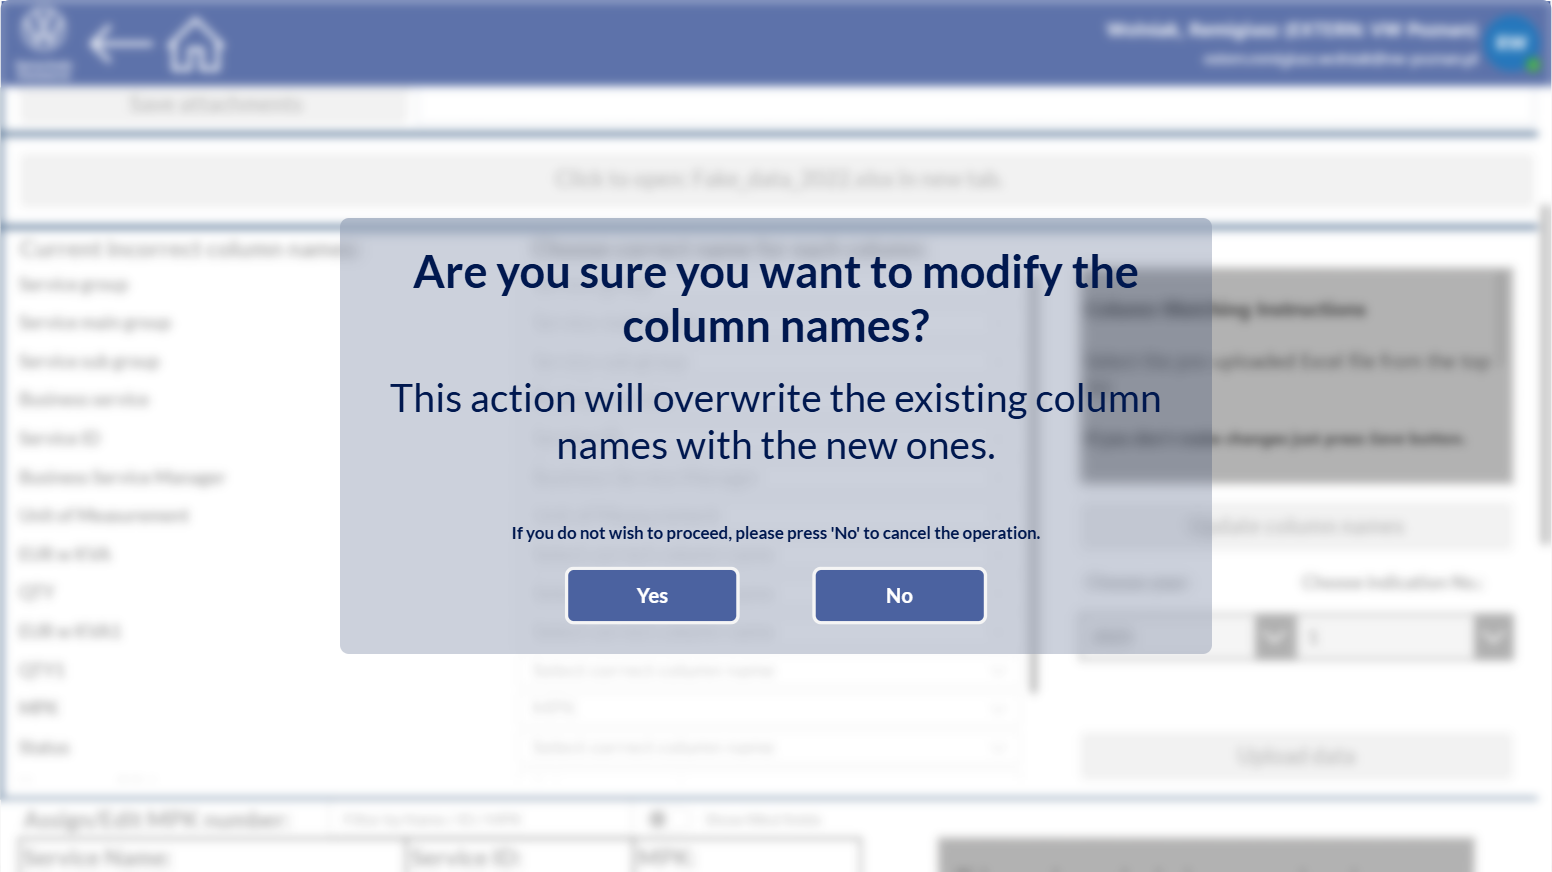
\includegraphics[width=\linewidth]{figures/CorrectHeadersPopup.png}
%         \caption{Zapytanie o poprawność nazw kolumn}
%         \label{fig:CorrectHeadersPopup}
%     \end{minipage}\hfill
%     % Drugi obrazek
%     \begin{minipage}{0.48\textwidth}
%         \centering
%         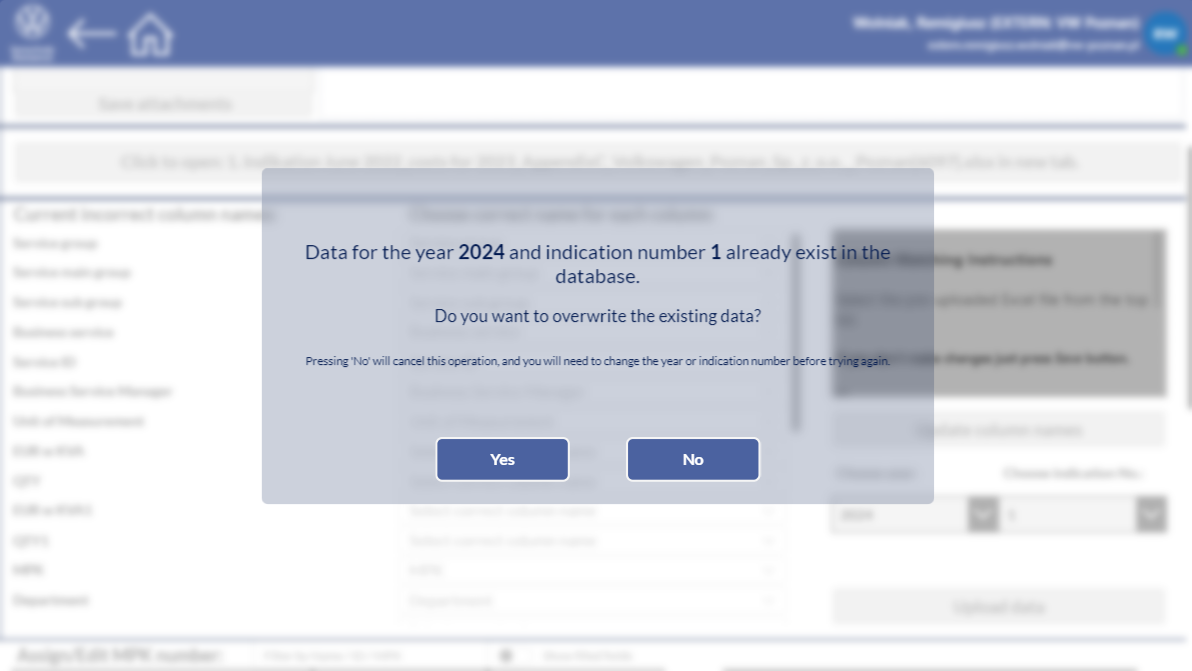
\includegraphics[width=\linewidth]{figures/DoUWantToOverwrite.png}
%         \caption{Zapytanie o nadpisanie danych}
%         \label{fig:DoYouWantToOverwrite}
%     \end{minipage}
%     \label{fig:obrazki}
% \end{figure}

Kiedy użytkownik upewni się, że wszystkie dane są poprawne i zatwierdzi operację, system przystępuje do importu danych. W tym celu zostaje wywołany kolejny przepływ w programie Power Automate, który przypisuje informacje do odpowiednich list w bazie danych, upewniając się jednocześnie, że nie zostaną dodane duplikaty rekordów.

\noindent Przepływ ten jest bardzo rozbudowany, dlatego zamiast widoku edytora Power Automate na rysunku \ref{fig:flowchart} przedstawiono schemat blokowy, reprezentujący kolejność wykonywania poszczególnych kroków. Został on uproszczony, ponieważ bloki umieszczone w błękitnych ramkach powinny być powielone do trzech równoległych gałęzi. Wynika to z faktu, że dla wszystkich list procedura jest identyczna, różnią się m.in. nazwy list użyte w strukturze żądań HTTP. Ponadto elementy, przedstawione z wykorzystaniem pomarańczowej, przerywanej ramki znajdują się w głęzi dotyczącej listy kwot. Odpowiadają one za pobieranie i przepisywanie numeru MPK z poprzedniego roku.


% Zmodyfikowane style z dodaną czcionką \large
\tikzstyle{startstop} = [rectangle, rounded corners, minimum width=3cm, minimum height=1cm, text centered, line width=2pt, draw={rgb,255:red,116; green,39; blue,116}, fill={rgb,255:red,234; green,223; blue,234}]

\tikzstyle{processExcel} = [rectangle, minimum width=3cm, minimum height=1cm, text centered, line width=2pt, draw={rgb,255:red,16; green,124; blue,65}, fill=ForestGreen!80]

\tikzstyle{Variable} = [rectangle, minimum width=3cm, minimum height=1cm, text centered, line width=2pt, draw={rgb,255:red,119; green,11; blue,214}, fill={rgb,255:red,171; green,104; blue,230}]

\tikzstyle{Data} = [rectangle, minimum width=3cm, minimum height=1cm, text centered, line width=2pt, draw={rgb,255:red,140; green,108; blue,255}, fill={rgb,255:red,166; green,141; blue,255}]

\tikzstyle{SP} = [rectangle, minimum width=3cm, minimum height=1cm, text centered, line width=2pt, draw={rgb,255:red,3 ; green,108; blue,112}, fill={rgb,255:red,39; green,181; blue,194}, align=center]

\tikzstyle{decision} = [diamond, minimum width=3cm, minimum height=1cm, text centered, draw=black, fill=green!30]

\tikzstyle{decision} = [diamond, minimum width=3cm, minimum height=1cm, text centered, draw=black, fill=green!30]
\tikzstyle{arrow} = [thick,->,>=stealth]
\tikzstyle{data} = [parallelogram, minimum width=3cm, minimum height=1cm, text centered, draw=black, fill=yellow!30]
\begin{figure}
    \resizebox{0.95\textwidth}{!}{%
        
\begin{tikzpicture}[node distance=3cm]
   
% Start node
\node (start) [startstop, text width=8cm, align=center] {\textbf{Trigger: Power Apps} \\[4pt]
\begin{tabular}{@{}cc@{}}
    FileName (string) & Year (number) \\
    IndicationNo (number) & Overwrite (bool) \\
\end{tabular}};

% Process nodes
\node (getTables) [processExcel, below of=start, fill=ForestGreen!80, text width=6cm, align=center, yshift=0.5cm] {\textbf{Get Tables} \\[4pt]
(from Excel with name \textit{FileName})};

\node (initializeVars) [Variable, align=center, text width=12cm, below of=getTables, yshift=-0.5cm] {
\textbf{Initialize Variables:}\\[4pt]
\begin{tabular}{@{}ll@{}}
- ExcelFile (Array) & - ItemsAddedToListaUslug (String) \\
- ItemsAddedToListaKwot (String) & - ItemsAddedToListaIndykacji (String) \\
- BatchRequestHeader (String) & - EndOfBatchRequest (String) \\
- Errors (String) \\
\end{tabular}
};


% Loop
% Twój niestandardowy bloczek jako węzeł
\node (applyToEach) [draw=none, inner sep=0pt, below of=initializeVars, below of=initializeVars, yshift=1.5cm] {%
    \begin{tikzpicture}[baseline]
        \draw [fill={rgb,255:red,152; green,171; blue,193}, draw={rgb,255:red,72; green,105; blue,145}, line width=2pt, dashed] (0,0) rectangle (5.5,-3.5);
        \draw [Variable, text width=4.5cm] (0.25,-1.5) rectangle node {\normalsize \textbf{Set Variable} \\[4pt]
        ExcelFile = TableContent} (5.25,-2.75);
        \node [font=\normalsize] at (2.75,-0.5) {\textbf{Apply to each}};
        \draw [processExcel] (0.25,-0.75) rectangle node {\normalsize \textbf{List rows present in table}} (5.25,-1.5);
    \end{tikzpicture}
};

% Select Columns
\node (selectCols) [Data, below of=applyToEach, text width=6cm, align=center] {\textbf{Select Columns from Excel}};

\node (Condition1) [rectangle, minimum width=3cm, minimum height=1cm, text centered, line width=2pt, draw={rgb,255:red,72; green,79; blue,88}, fill={rgb,255:red,149; green,153; blue,158},below of=selectCols, yshift=1cm, text width = 4cm] {\textbf{Condition 1}\\[4pt] \textit{Overwrite} == false};

\coordinate (belowCondition1) at ($(Condition1.south) - (0,2cm)$);


\node (ComplexNode) [draw=none, inner sep=0pt, anchor=north] at (Condition1.south) {%
    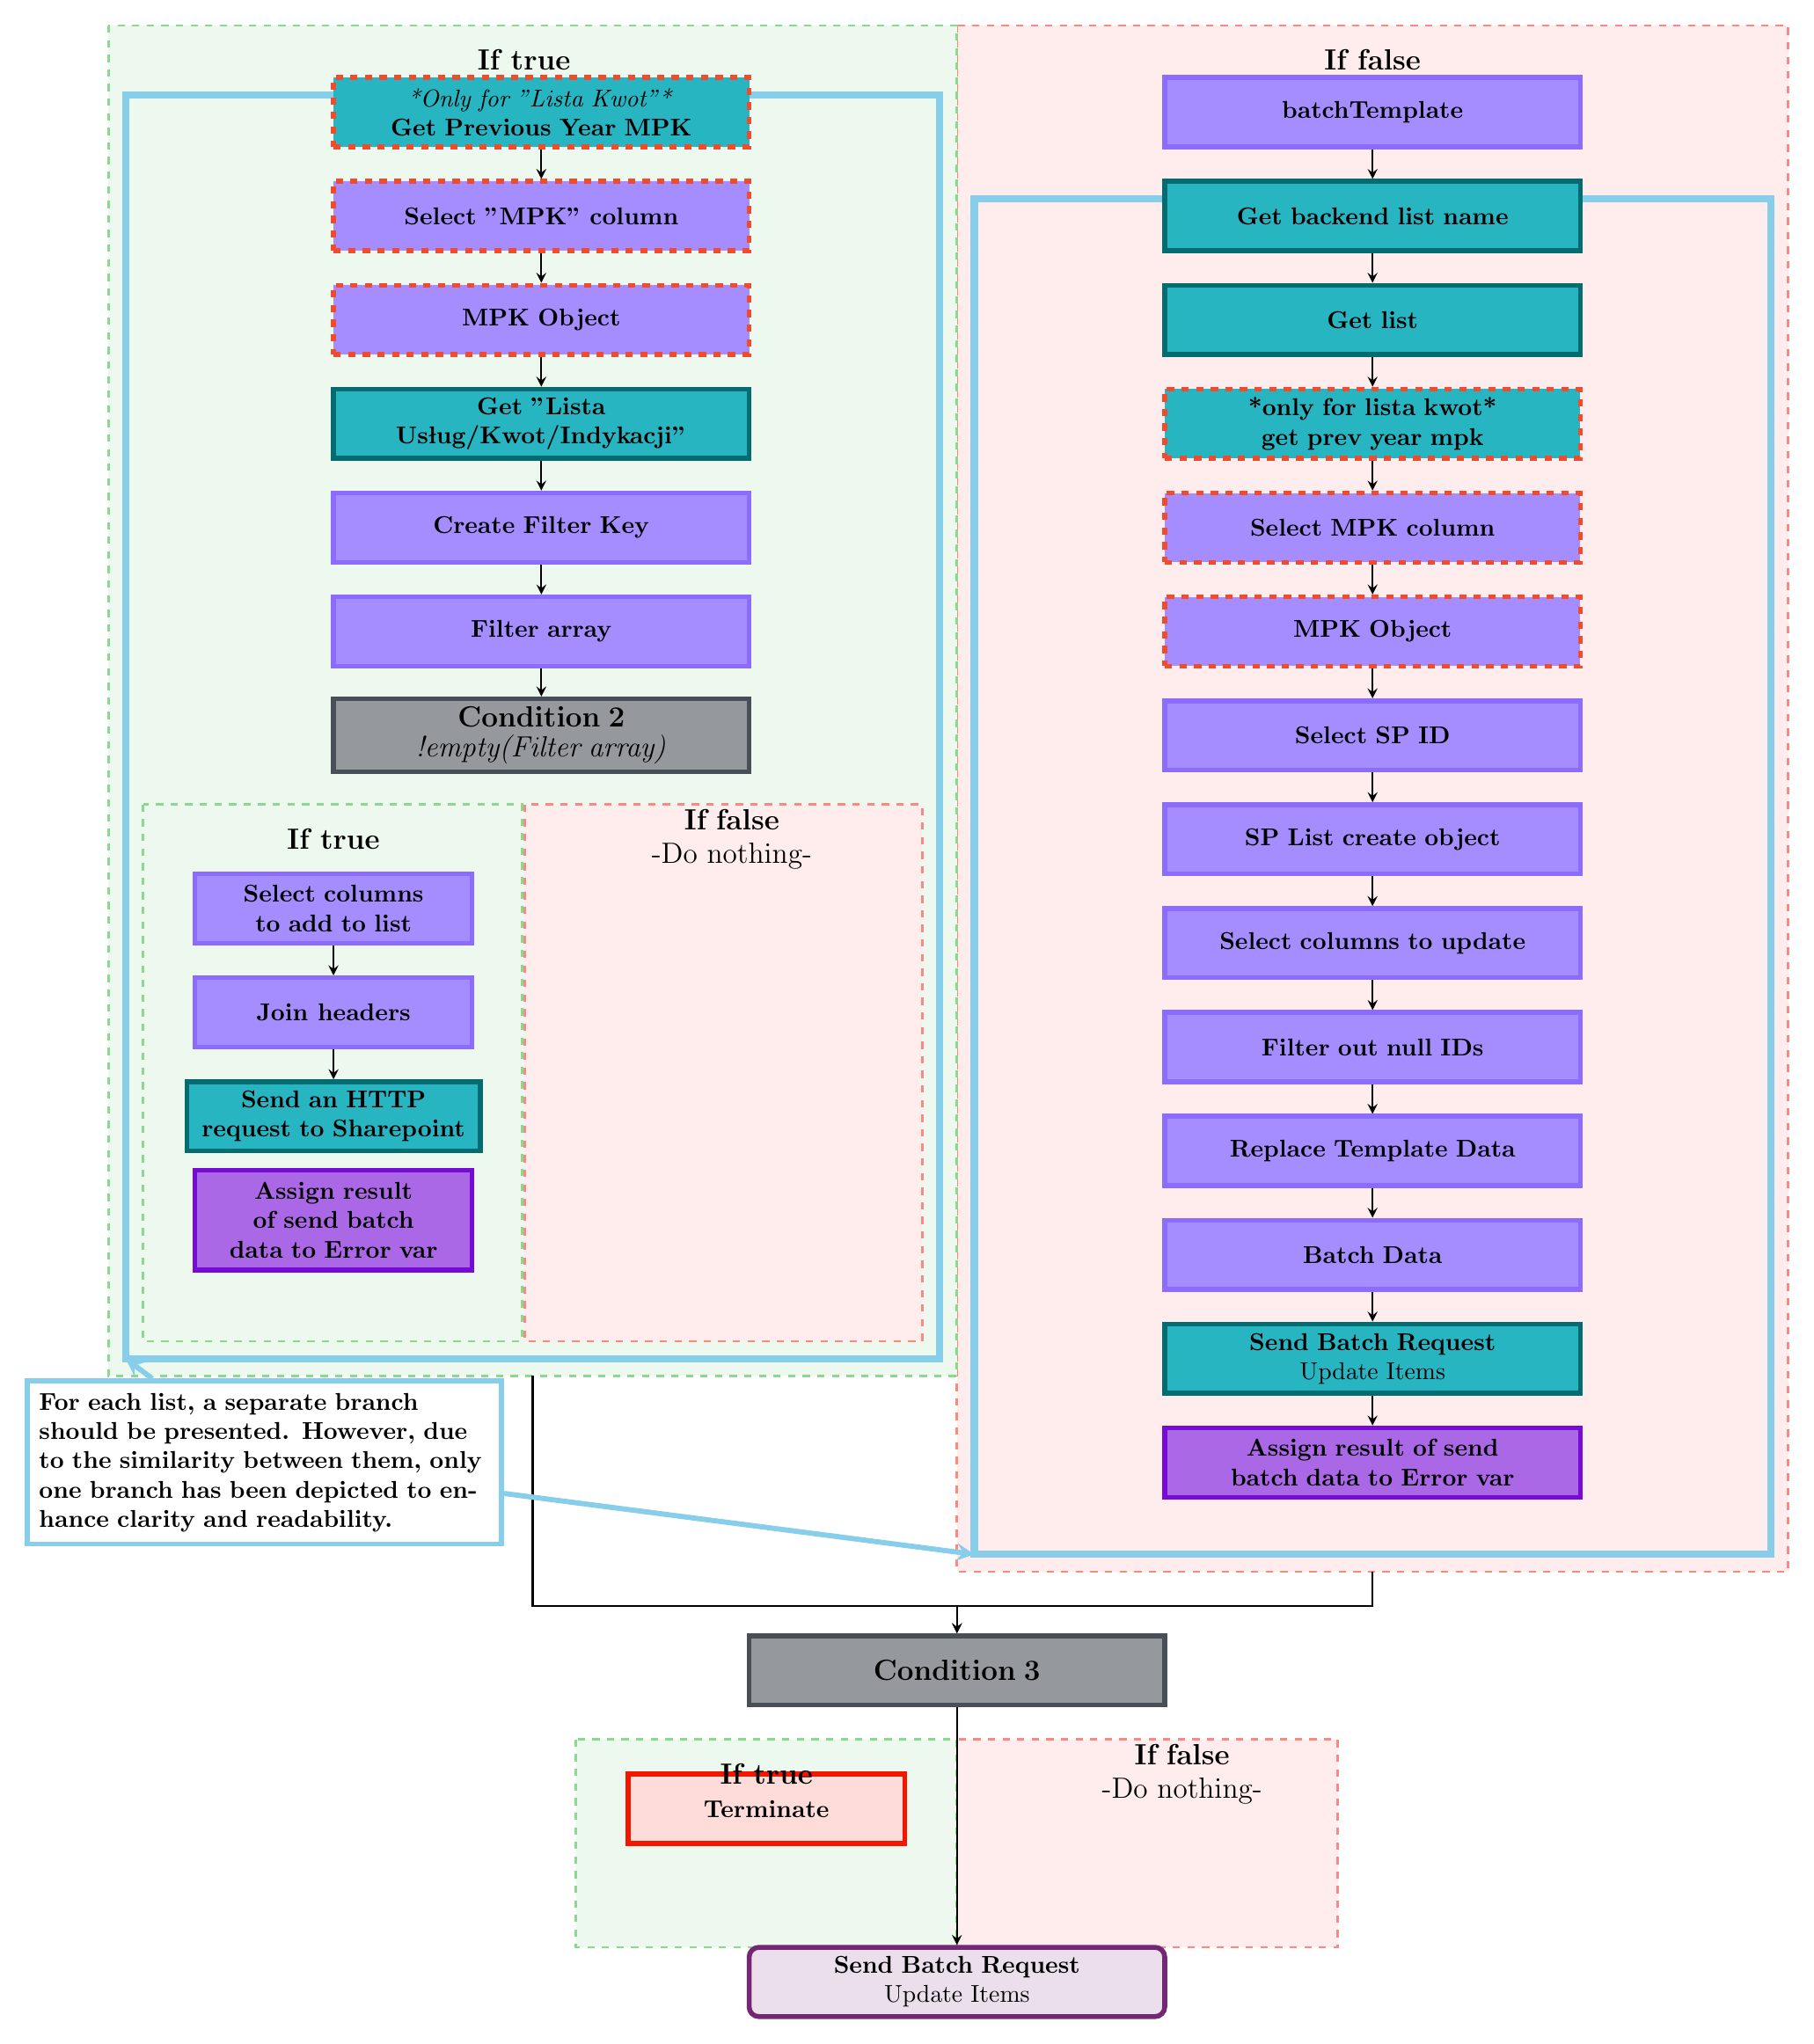
\begin{tikzpicture}[baseline]
\draw [ color={rgb,255:red,251; green,137; blue,129} , fill={rgb,255:red,254; green,237; blue,236}, line width=1pt , dashed] (2,23.75) rectangle  node {}  (14,1.425); %false
\draw [ color={rgb,255:red,136; green,218; blue,141} , fill={rgb,255:red,237; green,249; blue,238}, line width=1pt , dashed] (-10.25,23.75) rectangle  node {}  (2,4.25); %true
\draw [ color=SkyBlue, line width=3pt] (2.25,21.25) rectangle  node {}  (13.75,1.675); %false
\draw [ color=SkyBlue, line width=3pt] (-10,22.75) rectangle  node {}  (1.75,4.5); %true

\node (true1) [SP, dashed, minimum width=6cm, text width=5cm, draw=RedOrange] at (-4,22.5) {\normalsize \emph{*Only for "Lista Kwot"*}\\ \textbf{Get Previous Year MPK}};
\node (true2) [Data, minimum width=6cm, text width=5cm,dashed, draw=RedOrange] at (-4,21) {\normalsize \textbf{Select "MPK" column}};
\node (true3) [Data, minimum width=6cm, text width=5cm,dashed, draw=RedOrange] at (-4,19.5) {\normalsize \textbf{MPK Object}};
\node (true4) [SP, minimum width=6cm, text width=5cm, text width=5cm] at (-4,18) {\normalsize \textbf{Get "Lista Usług/Kwot/Indykacji"}};
\node (true5) [Data, minimum width=6cm, text width=5cm] at (-4,16.5) {\normalsize \textbf{Create Filter Key}};
\node (true6) [Data, minimum width=6cm, text width=5cm] at (-4,15) {\normalsize \textbf{Filter array}};

\draw [ color={rgb,255:red,136; green,218; blue,141} , fill={rgb,255:red,237; green,249; blue,238}, line width=1pt , dashed] (-9.75,12.5) rectangle  node {}  (-4.28,4.75);
\node (true11) [Data, minimum width=4cm, text width=3cm] at (-7,11) {\normalsize \textbf{Select columns to add to list}};
\node (true12) [Data, minimum width=4cm] at (-7,9.5) {\normalsize \textbf{Join headers}};
\node (true13) [SP, minimum width=4cm, text width=4cm] at (-7,8) {\normalsize \textbf{Send an HTTP request to Sharepoint}};
\node (true14) [Variable, minimum width=4cm, text width=3.5cm, inner sep=5pt] at (-7,6.5) { \textbf{Assign result of send batch data to Error var}};
\draw [ color={rgb,255:red,251; green,137; blue,129} , fill={rgb,255:red,254; green,237; blue,236}, line width=1pt , dashed] (-4.24,12.5) rectangle  node {}  (1.5,4.75);
\node (Condition2) [rectangle, minimum width=3cm, minimum height=1cm, text centered, line width=2pt, draw={rgb,255:red,72; green,79; blue,88}, fill={rgb,255:red,149; green,153; blue,158}, minimum width=6cm, text width=5cm] at (-4,13.5) {\large \textbf{Condition 2}\\ \emph{!empty(Filter array)}};
\node [font=\large] at (-4.25,23.25) {\textbf{If true}};
\node [font=\large] at (8,23.25) {\textbf{If false}};
\node [font=\large] at (-7,12) {\textbf{If true}};
\node [font=\large, text width=4cm, align=center] at (-1.25,12) {\textbf{If false}\\-Do nothing-};



\node (false1) [Data, minimum width=6cm, text width=5cm] at (8,22.5) { \textbf{batchTemplate}};
\node (false2) [SP, minimum width=6cm, text width=5cm] at (8,21) { \textbf{Get backend list name}};
\node (false3) [SP, minimum width=6cm, text width=5cm] at (8,19.5) { \textbf{Get list}};
\node (false4) [SP, minimum width=6cm, text width=5cm,dashed, draw=RedOrange] at (8,18) { \textbf{*only for lista kwot* \\ get prev year mpk}};
\node (false5) [Data, minimum width=6cm, text width=5cm,dashed, draw=RedOrange] at (8,16.5) { \textbf{Select MPK column}};
\node (false6) [Data, minimum width=6cm, text width=5cm,dashed, draw=RedOrange] at (8,15) { \textbf{MPK Object}};
\node (false7) [Data, minimum width=6cm, text width=5cm] at (8,13.5) {\textbf{Select SP ID}};
\node (false8) [Data, minimum width=6cm, text width=5cm] at (8,12) { \textbf{SP List create object}};
\node (false9) [Data, minimum width=6cm, text width=5cm] at (8,10.5) { \textbf{Select columns to update}};
\node (false10) [Data, minimum width=6cm, text width=5cm] at (8,9) { \textbf{Filter out null IDs}};
\node (false11) [Data, minimum width=6cm, text width=5cm] at (8,7.5) { \textbf{Replace Template Data}};
\node (false12) [Data, minimum width=6cm, text width=5cm] at (8,6) { \textbf{Batch Data}};
\node (false13) [SP, minimum width=6cm, text width=5cm] at (8,4.5) { \textbf{Send Batch Request}\\ Update Items};
\node (false14) [Variable, minimum width=6cm, text width=5cm] at (8,3) { \textbf{Assign result of send batch data to Error var}};

\draw [ color={rgb,255:red,251; green,137; blue,129} , fill={rgb,255:red,254; green,237; blue,236}, line width=1pt , dashed] (2,-1) rectangle  node {}  (7.5,-4);
\draw [ color={rgb,255:red,136; green,218; blue,141} , fill={rgb,255:red,237; green,249; blue,238}, line width=1pt , dashed] (-3.5,-1) rectangle  node {}  (2,-4);
\node[Data, minimum width=4cm, draw={rgb,255:red,244; green,23; blue,0} , fill={rgb,255:red,253; green,220; blue,217}] at (-0.75,-2) {\normalsize \textbf{Terminate}};
\node (Condition3) [rectangle, minimum width=3cm, minimum height=1cm, text centered, line width=2pt, draw={rgb,255:red,72; green,79; blue,88}, fill={rgb,255:red,149; green,153; blue,158}, minimum width=6cm, text width=5cm] at (2,0) {\large \textbf{Condition 3}};
    \node [font=\large] at (-0.75,-1.5) {\textbf{If true}};
\node [font=\large, text width=4cm, align=center] at (5.25,-1.5) {\textbf{If false}\\-Do nothing-};

\node (stop) [startstop, minimum width=6cm, text width=5cm] at (2,-4.5) { \textbf{Send Batch Request}\\ Update Items};
\node (annotation) [rectangle,text width=6.5cm, draw=SkyBlue,line width=0.75mm, inner sep=5pt] at (-8,3) {\textbf{For each list, a separate branch should be presented. However, due to the similarity between them, only one branch has been depicted to enhance clarity and readability.
}};
%Arrows
\draw [arrow] (true1) -- (true2);
\draw [arrow] (true2) -- (true3);
\draw [arrow] (true3) -- (true4);
\draw [arrow] (true4) -- (true5);
\draw [arrow] (true5) -- (true6);
\draw [arrow] (true6) -- (Condition2);

\draw [arrow] (true11) -- (true12);
\draw [arrow] (true12) -- (true13);

\draw [arrow] (false1) -- (false2);
\draw [arrow] (false2) -- (false3);
\draw [arrow] (false3) -- (false4);
\draw [arrow] (false4) -- (false5);
\draw [arrow] (false5) -- (false6);
\draw [arrow] (false6) -- (false7);
\draw [arrow] (false7) -- (false8);
\draw [arrow] (false8) -- (false9);
\draw [arrow] (false9) -- (false10);
\draw [arrow] (false10) -- (false11);
\draw [arrow] (false11) -- (false12);
\draw [arrow] (false12) -- (false13);
\draw [arrow] (false13) -- (false14);
\draw [arrow] (Condition3) -- (stop);



\draw [arrow] (-4.125,4.25) -- +(0,-3.325) -- +(6.125,-3.325) --(Condition3);
\draw [arrow] (8,1.425) -- +(0,-0.5) -- +(-6,-0.5) --(Condition3);
\draw [arrow, line width=0.75mm, SkyBlue] (annotation) -- (-10,4.5);
\draw [arrow, line width=0.75mm, SkyBlue] (annotation) -- (2.25,1.675);
\end{tikzpicture}

};
\draw [arrow] (start) -- (getTables);
\draw [arrow] (getTables) -- (initializeVars);
\draw [arrow] (initializeVars) -- (applyToEach);
\draw [arrow] (applyToEach) -- (selectCols);
\draw [arrow] (selectCols) -- (Condition1);




\end{tikzpicture}

    }
    \caption{Schemat blokowy procesu importu danych z arkusza kalkulacyjnego do bazy danych}
    \label{fig:flowchart}
\end{figure}

\pagebreak
Poniżej wyjaśniono działanie poszczególnych bloków znajdujących się na schemacie. Elementy oznaczone symbolem (\textasteriskcentered) odnoszą się do bloków otoczonych pomarańczową, przerywaną ramką.
\begin{enumerate}
    \item Blok \textbf{Trigger: Power Apps} jest wyzwalaczem działania przepływu. Uruchamia się wtedy, gdy użytkownik wciśnie przycisk w aplikacji. Jako parametry wejściowe przyjmuje nazwę pliku, rok oraz numer indykacji, które mają być przypisane do danych oraz informacje czy nadpisać istniejące rekordy czy też nie.

    \item \textbf{Get Tables} pobiera nazwy wszystkich tabel z pliku o nazwie przekazanej do wyzwalacza (każdy plik powinien zawierać jedną tabelę, ale w Power Automate trzeba pobrać wszystkie możliwe).
    \item Funkcja \textbf{Initialize variable} tworzy następujące zmienne:
          \begin{itemize}
              \item \emph{ExcelFile} -- zmienna tablicowa, przechowująca dane z arkusza,
              \item \emph{ItemsAddedToListaUsług/Kwot/Indykacji} -- te zmienne przechowują \emph{ciało żądania HTTP}, które jest konstruowane w trakcie działania przepływu.
              \item \emph{BatchRequestHeader} oraz \emph{EndOfBatchRequest} -- przechowują one stałe nagłówki i stopkę żądania HTTP, które są wspólne dla wszystkich zapytań.
          \end{itemize}
    \item Pętla \textbf{Apply to each}, dodana automatycznie przez Power Automate, iteruje po nazwach tabel pobranych z pliku, a następnie dla każdej z nich przepisuje dane do zmiennej \emph{ExcelFile}.
    \item Funkcja \textbf{Select Columns from Excel} pozwala na kształtowanie danych. Jako wejście przyjmuje ona dane z \emph{ExcelFile}, a następnie mapuje wartości tej zmiennej do wybranych kluczy. Dzięki temu można odwołać się do dowolnej kolumny danych.
    \item Blok \textbf{Condition 1} sprawdza czy wartość \emph{Overwrite} jest równa \emph{false}.
          Jeśli tak, to wykonywane są instrukcje wewnątrz bloku \emph{True}. Gałąź ta odpowiada za dopisanie nowych danych do bazy. W tym celu wykonywane są następujące instrukcje:
          \begin{itemize}[label=\textasteriskcentered]
              \item \textbf{Get Previous Year MPK} -- pobiera elementy z listy kwot dla roku wcześniejszego niż przekazany w parametrze wejściowym,
              \item \textbf{Select "MPK" column} -- jako wejście przyjmuje odpowiedź z bloku poprzedniego, ale zamiast przypisywania wartości do klucza zawiera następujące wyrażenie:

                    \begin{center}
                        \texttt{concat("",item()?['Service\_ID'],'":',item())}
                    \end{center}

                    \emph{item()} odwołuje się do pojedynczego elementu danych wejściowych, zatem to wyrażenie tworzy strukturę obiektów, gdzie nazwą obiektu jest \emph{Service\_ID}, natomiast jako właściwości obiektu przypisane są dane z arkusza odpowiadające tej usłudze.
              \item \textbf{MPK Object} przekształca strukturę utworzoną w poprzednim kroku na listę obiektów JSON.
          \end{itemize}

          \begin{itemize}
              \item\textbf{Get "Lista Usług/Kwot/Indykacji"} -- pobiera pełną listę rekordów z odpowiedniej listy w bazie danych.
              \item \textbf{Create Filter Key} -- tworzy klucz filtrujący. Dla listy usług nie jest on wymagany, w przypadku listy kwot kluczem jest rok przekazany w parametrze wejściowym, natomiast dla listy indykacji jest to rok oraz numer indykacji połączone w jeden ciąg znaków.
              \item \textbf{Filter array} -- jest blokiem wykorzystywanym do porównania elementów dla danego roku i indykacji na liście SharePoint z elementami w arkuszu. Ma on za zadanie zwrócić tablicę z elementami unikalnymi dla arkusza.
              \item \textbf{Condition 2} sprawdza, czy tablica zwrócona przez \emph{Filter array} nie jest pusta. Jeżeli nie zawiera ona unikatowych elementów, to przepływ kończy działanie, jednak jeśli tablica zawiera unikatowe elementy, to przepływ przechodzi do kolejnego kroku w gałęzi \emph{True}.
              \item \textbf{Select columns to add to list} -- mapuje informacje z arkusza do kluczy odpowiadających strukturze każdej z list w bazie danych.
              \item \textbf{Join headers} -- konwertuje tablicę powstałą w poprzednim kroku na ciąg znaków, będący ciałem żądania HTTP. Instrukcja ta zmienia separator między wierszami tabeli ze średnika na nagłówek, który musi znajdować się między każdym wysłanym zestawem danych. Dla każdej z list jest on inny.
              \item \textbf{Send an HTTP request to SharePoint} -- wysyła kompletne żądanie HTTP do odpowiedniej listy w bazie danych. Wysyłane żądanie zawiera:
                    \begin{itemize}
                        \item Nagłówek otwierający żądanie -- \emph{BatchRequestHeader},
                        \item Ciało żądania powstałe w kroku wcześniej -- wynik \emph{Join headers},
                        \item Stopkę żądania -- \emph{EndOfBatchRequest}.
                    \end{itemize}
              \item \textbf{Assign result of send batch data to Error var} -- przypisuje odpowiedź serwera na wysłane żądanie w celu późniejszej analizy.
          \end{itemize}

          Kiedy jednak wartość zmiennej \emph{Overwrite} wynosi \emph{True}, oznacza to, że istniejące rekordy mają zostać zaaktualizowane. Przeplyw przechodzi do gałęzi \emph{False} i wykonuje następujące kroki:
          \begin{itemize}
              \item \textbf{batchTemplate} -- tworzy wspólny szablon żądania HTTP.
              \item \textbf{Get backend list name} -- pobiera wewnętrzną nazwę listy SharePoint. Jest to konieczne, ponieważ w żądaniu HTTP należy ostrożnie używać znaków specjalnych.
              \item \textbf{Get list} -- odczytuje dane z każdej z list.
          \end{itemize}
          \begin{itemize}[label=\textasteriskcentered]
              \item Funkcje \textbf{Get Previous Year MPK}, \textbf{Select "MPK" column} oraz \textbf{MPK Object} wykonują te same zadania, co w uprzednio omówionym scenariuszu.
          \end{itemize}
          \begin{itemize}
              \item Kroki \textbf{Select SP ID} i \textbf{SP List create object} działają podobnie jak mechanizm pobierania numerów MPK z roku poprzedniego, z tą różnicą, że mapują one identyfikatory wewnętrzne elementów listy SharePoint. Jest to konieczne, ponieważ w celu aktualizacji rekordu należy odwołać się do niego względem tego właśnie identyfikatora, a nie np. nazwy lub \emph{Service\_ID}.
              \item \textbf{Select columns to update} -- przydziela informacje z odpowiednich kolumn do odpowiednich list.
              \item \textbf{Filter out null IDs} -- odfiltrowuje elementy, które nie mają przypisanego identyfikatora SharePoint. Gdyby nie ten krok, próba aktualizacji rekordu bez identyfikatora zakończyłaby się błędem.
              \item  \textbf{Replace Template Data} -- wstawia wybrane informacje do szablonu żądania HTTP.
              \item \textbf{batchData} -- w kroku tym znaki specjalne są zakodowane procentowo\footnote{\emph{Kodowanie procentowe} -- metoda reprezentowania znaków specjalnych w adresach URL w formie zgodnej z protokołem HTTP. Polega na zastępowaniu niebezpiecznych lub niedozwolonych znaków ich odpowiednikami w postaci procentowego kodu, który składa się z symbolu "\%" i dwóch cyfr szesnastkowych reprezentujących kod ASCII danego znaku.} (znane również jako \emph{kodowanie URL}). Jest to wymagane, aby uniknąć niepożądanych błędów, związanych ze znakami specjalnymi.
              \item \textbf{Send Batch Request} -- wysyła żądanie aktualizacji danych do SharePoint.
              \item \textbf{Assign result of send batch data to Error var} -- przypisuje odpowiedź serwera na wysłane żądanie w celu późniejszej analizy.
          \end{itemize}

    \item \textbf{Condition 3} sprawdza, czy zmienna \emph{Errors} zawiera jakiekolwiek kody błędów. Jeśli tak, to przepływ zostaje przerwany, w przeciwnym wypadku zwracana jest informacja do aplikacji, że zapis danych zakończył się powodzeniem.
\end{enumerate}

\subsection{Uzupełnianie numerów MPK}
Ostatnią funkcją tego ekranu jest możliwość uzupełniania lub edycji numerów MPK. W tym celu ponownie wykorzystano galerię, która tym razem składa się z trzech kolumn. Dwie pierwsze kolumny zawierają pola tekstowe (\definicja{Label}), które prezentują nazwę usługi oraz odpowiadający jej identyfikator. Ostatnia kolumna zawiera pole danych wejściowych (\definicja{TextInput}), do którego użytkownik wprowadza odpowiedni numer MPK. Nad galerią znajduje się dodatkowe pole, w którym można wpisać kryteria filtrowania, takie jak nazwa, identyfikator bądź numer MPK. Obok pól filtracji znajduje się przełącznik (\definicja{Toggle}), który umożliwia wyświetlenie usług z przypisanym już numerem MPK. Istniejące numery MPK wyświetlają się jako domyślny tekst kontrolki \emph{TextInput} i mogą być edytowane. Ostatnim elementem ekranu jest pole tekstowe, informujące użytkownika o liczbie usług bez przypisanego miejsca powstawania kosztów.
% \begin{figure}[t]
%     \centering
%     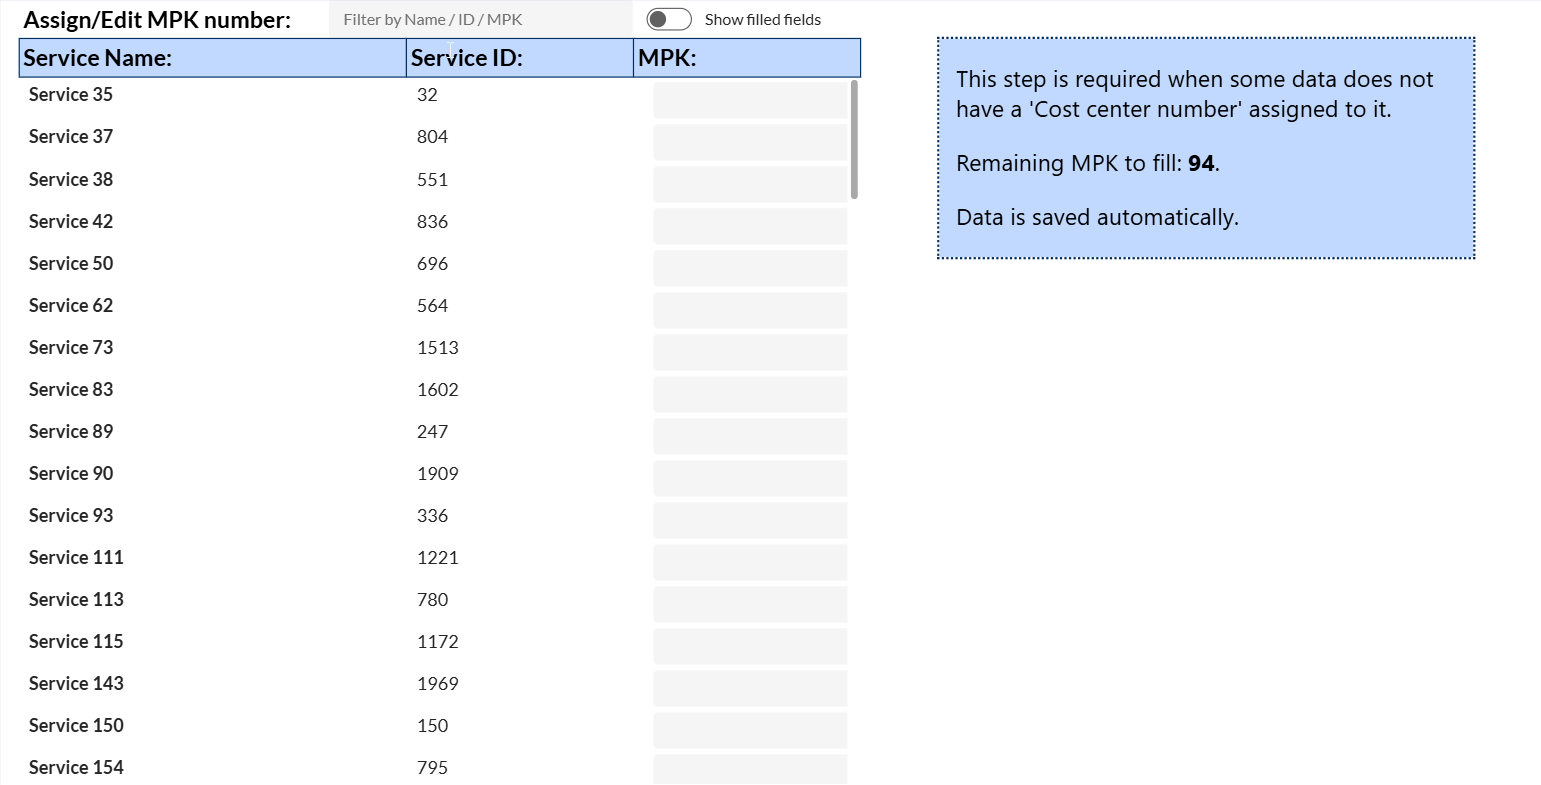
\includegraphics[width=\textwidth]{figures/FillMPKForm.png}
%     \caption{Formularz wypełniania/edycji numerów MPK}
%     \label{fig:fillmpkform}
% \end{figure}